\section{Algorithmic Approaches}

\begin{definition}
The $m \times n$ \term{comparability grid} is a graph $G = (V,E)$ with
\begin{align}
    V &= \{(i,j) \mid i \in [m], j \in [n]\} \\
    \label{eq:comp-grid-edges}
    E &= \{ \{(i_1,j_1),(i_2,j_2)\} \mid (i_1,j_1),(i_2,j_2) \in V, i_2 \geq i_1, j_2 \geq j_1. \}
\end{align}
In other words, $m$ rows and $n$ columns with edges defined by the partial order $\leq$. Denote such graphs as $\CGrid_{m \times n}$. Let $\CGrid$ denote the family of all such graphs. By abuse of notation, let it also denote the resource state of all graph states corresponding to comparability grids.
\end{definition}

\begin{example}
Figure 3 shows the $3 \times 3$ comparability grid:
\begin{figure}[H]
\centering
\begin{tikzpicture}[
  scale=1.7,
  every node/.style={circle, fill=black, inner sep=1.5pt},
  edge/.style={line width=0.5pt}
]
\node (v11) at (1,1) {};
\node (v12) at (1,2) {};
\node (v13) at (1,3) {};
\node (v21) at (2,1) {};
\node (v22) at (2,2) {};
\node (v23) at (2,3) {};
\node (v31) at (3,1) {};
\node (v32) at (3,2) {};
\node (v33) at (3,3) {};

\draw[edge] (v11) -- (v12);
\draw[edge] (v11) -- (v21);
\draw[edge] (v11) -- (v22);
\draw[edge] (v11) -- (v23);
\draw[edge] (v11) -- (v32);

\draw[edge] (v12) -- (v13);
\draw[edge] (v12) -- (v22);
\draw[edge] (v12) -- (v23);

\draw[edge] (v13) -- (v23);

\draw[edge] (v21) -- (v22);
\draw[edge] (v21) -- (v31);
\draw[edge] (v21) -- (v32);

\draw[edge] (v22) -- (v23);
\draw[edge] (v22) -- (v32);

\draw[edge] (v23) -- (v33);
\draw[edge] (v31) -- (v32);
\draw[edge] (v32) -- (v33);

\draw[edge] (v11) to[bend left=20] (v13);
\draw[edge] (v21) to[bend left=20] (v23);
\draw[edge] (v31) to[bend left=20] (v33);

\draw[edge] (v11) to[bend right=20] (v31);
\draw[edge] (v12) to[bend right=20] (v32);

\draw[edge] (v11) to[bend right=20] (v33);
\draw[edge] (v12) to[bend right=20] (v33);
\draw[edge] (v13) to[bend right=20] (v33);

\draw[edge] (v21) to[bend right=20] (v33);
\draw[edge] (v22) to[bend right=20] (v33);

\node[draw=none, fill=none, inner sep=0pt, anchor=east] at ($(v13)+(-0.15,0)$) {$ (1,3)$};
\node[draw=none, fill=none, inner sep=0pt, anchor=west] at ($(v33)+(0.15,0)$) {$ (3,3)$};
\node[draw=none, fill=none, inner sep=0pt, anchor=east] at ($(v11)+(-0.15,0)$) {$ (1,1)$};
\node[draw=none, fill=none, inner sep=0pt, anchor=west] at ($(v31)+(0.15,0)$) {$ (3,1)$};
\end{tikzpicture}
\label{fig:comp-grid-example}
\caption{$\CGrid_{3 \times 3}$.}
\end{figure}

\end{example}

We dedicate the rest of this section to algorithmic approaches in determining the CQ-universality of the $\CGrid$ resource.

\subsection{Subsets of the Comparability Grid}

One idea it to ask how close ``vertex deletion'' can get us to universal quantum computation. Namely, can we delete vertices to get a $\Grid$? If not, how close can we get?

\begin{definition}
Define a subset of a $\CGrid$ state as the graph corresponding to a state in $\CGrid$ with some vertices measured in the $Z$ basis. Graph theoretically, a subset of a $\CGrid$ is a $\CGrid$ with some vertices removed (alongside any edges connected to said removed vertices).
\end{definition}

\begin{fact}
Any subset $H$ with $n$ vertices of any $\CGrid$ can be uniquely identified as a permutation of $[n]$, denoted $\pi \in S_n$. Denote this by $\pi(H)$. Similarly, let $H(\pi)$ denote the subgraph corresponding to $\pi$.
\begin{proof}
\note{This proof only works for finite subsets, but there is a need to define it for infinite-sized vertex subsets. }
Consider an arbitrary subset $H = (V,E)$ with $|V| = n$ of a fixed $\CGrid$ $G$. We claim this subgraph is isomorphic to the graph $H' = (V', E')$, where 
\begin{enumerate}
    \item $V' = \{ (x+\nicefrac{y}{n},y+\nicefrac{x}{n}) \mid (x,y) \in V \}$
    \item $E' = \{ \{(x_1+\nicefrac{y_1}{n},y_1+\nicefrac{x_1}{n}), (x_2+\nicefrac{y_2}{n},y_2+\nicefrac{x_2}{n})\} \mid \{(x_1,y_1), (x_2,y_2)\} \in E\}$.
\end{enumerate}
That is, $H'$ is the graph whose $x'$ and $y'$ values have been shifted rightwards and upwards, respectively. Since $|V| = n$, there is a clear bijection from $V$ to $V'$. The bijection between edges follows as $|E| = |E'|$.

We claim the data of $H'$ can be completely expressed as follows: Sort the vertices in $V'$ by their $x'$-coordinate. No two distinct vertices can share an $x'$ coordinate: We proceed by contradiction. If $x_1 = x_2$
\begin{align}
    x_1+\frac{y_1}{n} = x_2+\frac{y_2}{n}
    \implies 
    y_1 = y_2
\end{align}
but then they are not distinct vertices. If $x_1 \neq x_2$, without loss of generality let $x_1 > x_2$ so $x_1 = x_2 + c$, $c \in \N$. Then
\begin{align}
    x_1+\frac{y_1}{n} = x_2+\frac{y_2}{n}
    \implies 
    c = \frac{y_1}{n} - \frac{y_2}{n}
    \implies
    c = \frac{1}{n}(y_1 - y_2)
\end{align}
Since $y_1, y_2 \leq n$, the RHS $\leq 1$. Contradiction. No two distinct vertices share a $y'$ coordinate either, by a similar proof. Re-label each vertex by their order, from least to greatest, in both $x'$ and $y'$. Edges still form by the partial ordering rule in Equation \ref{eq:comp-grid-edges}. Reading the $x'$ coordinate as the index of a $n$-tuple and the $y'$ coordinate as the values, we obtain a permutation of $n$ as each $x'$, $y'$ is distinct.
\end{proof}
\end{fact}

\begin{fact}
Two subsets $H,H'$ of a $\CGrid$ may have $\pi(H) \neq \pi(H')$ yet $H = H'$ up to vertex relabeling.
\begin{proof}
Take subgraphs with vertices $V = \{(1,1), (1,2)\}$ and $V' = \{(1,1), (2,1)\}$ and their induced edges. The first has permutation $(1,2)$ and the second $(2,1)$ but the graphs are clearly isomorphic.
\end{proof}
\end{fact}

\begin{fact}
Let $\pi\in S_n$ and define its reverse-complement
\begin{align}
    \pi^{\mathrm{rc}}(i) := (n+1) - \pi(n+1-i).
\end{align}
Then the induced $\CGrid$ subgraphs satisfy $H(\pi)\cong H(\pi^{\mathrm{rc}})$.
\begin{proof}
Write vertices of $H(\pi)$ as $v_i=(i,\pi(i))$. Define a bijection
\begin{align}
    f: v_i \mapsto v'_{n+1-i} := \bigl(n+1-i,\; n+1-\pi(i)\bigr).    
\end{align}
The image vertex set is exactly $\{(k,\pi^{\mathrm{rc}}(k)) \mid k\in[n]\}$, so $f$ is a bijection from $V(H(\pi))$ to $V(H(\pi^{\mathrm{rc}}))$.
An edge in a comparability grid exists between $v_i$ and $v_j$ iff
\begin{align}
    (i-j)\bigl(\pi(i)-\pi(j)\bigr) > 0,    
\end{align}
equivalently $(i<j \ \&\ \pi(i)<\pi(j))$ or $(i>j \ \&\ \pi(i)>\pi(j))$. But under $f$ we have
\begin{align}
    (n+1-i)-(n+1-j) &= -(i-j),\\
    (n+1-\pi(i))-(n+1-\pi(j)) &= -(\pi(i)-\pi(j)),    
\end{align}
so the product $(i-j)(\pi(i)-\pi(j))$ is preserved. Hence $\{v_i,v_j\}$ is an edge iff $\{f(v_i),f(v_j)\}$ is an edge. Therefore $f$ is a graph isomorphism.
\end{proof}
\end{fact}

\begin{theorem}
\label{thm:subset-alg}
Let $\pi(H)$ denote a permutation of $n$ capturing the data of a finite subset $H = (V,E) \leq G$ with $|V|=n$, for some $G \in \CGrid$. The degree sequence of $\pi(H)$ can be constructed algorithmically in $O(n \log n)$ time and $O(n)$ space.
\begin{proof}
For any $\pi \in S_n$, let an \term{inversion} be a pair $(i,j)$, $i \neq j \in [n]$, such that 
\begin{align}
    i < j \text{ and } \pi[i] > \pi[j].
\end{align}
$(i,j)$ is a \term{non-inversion} if
\begin{align}
    i < j \text{ and } \pi[i] < \pi[j].
\end{align}
Since $i \neq j$, every $(i,j)$ is either an inversion or non-inversion. Thus
\begin{align}
    \#\text{non-inversions} = \binom{n}{2} - \#\text{inversions}.
\end{align}
At position $j \in [n]$ of the permutation, 
\begin{align}
    |\{i < j \mid \pi[i] < \pi[j]\}| = \text{prefixSum}(\pi[j] - 1).
\end{align}
Here, prefix sum refers to the number of indies with index $\leq j$ and value $\leq \pi[j]$. The $-1$ makes $\leq$ become $<$. In other words, for each $j$, we count the number of indices $i < j$ such that $\pi[i] < \pi[j]$.

It is well-known that a prefix sum can be computed in $\Theta(\log n)$ time using a binary index tree or Fenwick tree. Since there are $n$ iterations, the total time is $\Theta(n \log n)$. The Fenwick tree is the only allocation, and only needs $\Theta(n)$ more space.

Run the above procedure on the reverse of $\pi(H)$. This counts, for each $j$. the number of indices $i < j$ such that $\pi[i] > \pi[j]$. Adding the two values for each index gives the degree of the corresponding vertex. Denote this algorithm as \term{double inversion}.
\end{proof}
\end{theorem}

We use double-inversion rather than directly constructing the edges due to the following fact:

\begin{fact}
In a subgraph $H$ with $n$ vertices, there is at most $O(n^2)$ edges. Thus, enumerating the edges of some $\pi(H)$ cannot be better than $O(n^2)$ in the worst general case.
\end{fact}

Recall that our goal is to identify whether vertex deletion alone can get us to a subgraph isomorphic to some $\Grid$ graph. This is surprisingly true for $2 \times n$ grids for all $n \in \N$.

\begin{theorem}
The $2 \times n$ $\Grid$ is obtainable from a sufficiently large $\CGrid$ through vertex deletion alone.
\begin{proof}
Fix $G = \CGrid_{n \times n}$. Define the $i$th \term{anti-diagonal} as
\begin{align}
    A_n := \{ (i,j) \mid i + j = n + 1\}
\end{align}
For example, $A_1 = \{(1,1)\}$ and $A_2 = \{(1,2), (2,1)\}$. Delete all vertices not in some $A_j$ or $A_{j+1} \setminus \{(j,1),(1,j)\}$ for $j \in [n-1]$. The remaining vertices and induced edges form a $2 \times n$ grid:
\begin{figure}[H]
\centering
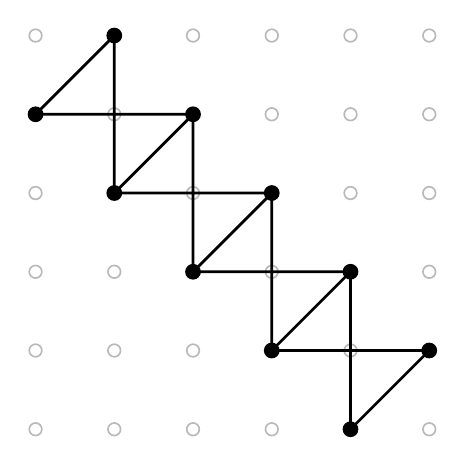
\begin{tikzpicture}[line cap=round, line join=round]

\foreach \x in {0,...,5} {
    \foreach \y in {0,...,5} {
    \draw[gray!55, line width=0.6pt] (\x,\y) circle[radius=0.08];
    }
}

\draw[black, line width=1.0pt]
    (0,4)--(1,5)
    (1,5)--(1,4)
    (0,4)--(1,4)--(2,4)
    (1,4)--(1,3)
    (1,3)--(2,4)
    (1,3)--(2,3)--(2,4)
    (2,3)--(2,2)
    (2,3)--(3,3)
    (2,2)--(3,3)
    (2,2)--(3,2)--(3,3)
    (3,2)--(3,1)
    (3,2)--(4,2)
    (3,1)--(4,2)
    (3,1)--(4,1)--(4,2)
    (4,1)--(4,0)
    (4,1)--(5,1)
    (4,0)--(5,1);

\foreach \p in {(0,4),(1,5),(1,3),(2,4),(2,2),(3,3),(3,1),(4,2),(4,0),(5,1)}{
    \fill[black] \p circle[radius=0.10];
}
\end{tikzpicture}
\caption{A $\Grid_{2 \times 5}$ in a $\CGrid_{6 \times 6}$.}
\label{fig:two-wide-grid-in-cgrid}
\end{figure}
To see that this is a grid, ``twist'' the above figure.
\end{proof}
\end{theorem}

However, the above pattern does not generalize for larger widths.

\begin{fact}
It is not possible to get a $\Grid_{3 \times n}$ subgraph from any size of $\CGrid$ using only vertex deletion.
\begin{proof}
Brute force using the algorithm described in Theorem \ref{thm:subset-alg}.
\end{proof}
\end{fact}

That said, we can get quite close to a grid:

\begin{definition}
\label{def:3n-subgrid}
Consider the following construction:
\begin{figure}[H]
\centering
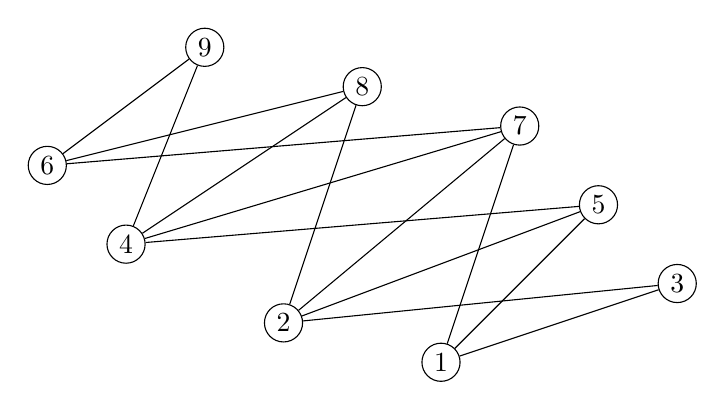
\begin{tikzpicture}
\tikzstyle{vertex}=[draw, circle, inner sep=2pt]
    \node[vertex] (6) at (0,3) {$6$};
    \node[vertex] (4) at (1,2) {$4$};
    \node[vertex] (9) at (2,4.5) {$9$};
    \node[vertex] (2) at (3,1) {$2$};
    \node[vertex] (8) at (4,4) {$8$};
    \node[vertex] (1) at (5,0.5) {$1$};
    \node[vertex] (7) at (6,3.5) {$7$};
    \node[vertex] (5) at (7,2.5) {$5$};
    \node[vertex] (3) at (8,1.5) {$3$};

    \draw (6) -- (9);
    \draw (6) -- (8);
    \draw (6) -- (7);
    
    \draw (4) -- (9);
    \draw (4) -- (8);
    \draw (4) -- (7);
    \draw (4) -- (5);
    
    \draw (2) -- (8);
    \draw (2) -- (7);
    \draw (2) -- (5);
    \draw (2) -- (3);
    
    \draw (1) -- (7);
    \draw (1) -- (5);
    \draw (1) -- (3);
    
\end{tikzpicture}
\label{fig:3n-compgraph}
\caption{A subset close to a $\Grid_{3 \times 3}$ from some large $\CGrid$ using only vertex deletion.}
\end{figure}
This forms the following subgrid:
\begin{figure}[H]
\centering
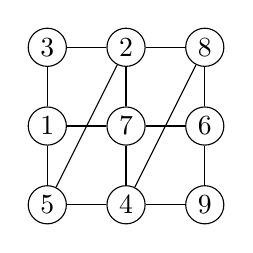
\begin{tikzpicture}
\tikzstyle{vertex}=[draw, circle, inner sep=2pt]
    \node[vertex] (1) at (0,1) {$1$};
    \node[vertex] (2) at (1,2) {$2$};
    \node[vertex] (3) at (0,2) {$3$};
    \node[vertex] (4) at (1,0) {$4$};
    \node[vertex] (5) at (0,0) {$5$};
    \node[vertex] (6) at (2,1) {$6$};
    \node[vertex] (7) at (1,1) {$7$};
    \node[vertex] (8) at (2,2) {$8$};
    \node[vertex] (9) at (2,0) {$9$};

    \draw (6) -- (9);
    \draw (6) -- (8);
    \draw (6) -- (7);
    
    \draw (4) -- (9);
    \draw (4) -- (8);
    \draw (4) -- (7);
    \draw (4) -- (5);
    
    \draw (2) -- (8);
    \draw (2) -- (7);
    \draw (2) -- (5);
    \draw (2) -- (3);
    
    \draw (1) -- (7);
    \draw (1) -- (5);
    \draw (1) -- (3);

\end{tikzpicture}
\label{fig:3n-subgrid}
\caption{Tileable $\Grid_{3 \times n}$ subgraph of $\CGrid$ with one additional edge every column.}
\end{figure}
This construction is tileable. That is, it generalizes to $\Grid_{3 \times n}$ provided a sufficiently large $\CGrid$.
\begin{proof}
\note{I had an extremely complicated proof. The crux of the issue is that every time a new column is added, we need to ensure that it can "fit" in between (in either the x or y dimension) some previous existing points. Since our points need to in $\N \times \N$, the simplest solution is to pre-allocate some gap between the nodes. However, this becomes extremely cumbersome very quickly.

An easier proof is to work graphically. That said, it would be great if the proof was in the ZX-representation of the $\CGrid$, as this may highlight some important identities and tricks usable for even higher widths.}
\end{proof}
\end{definition}

\subsection{The Width-3 Gadget}

The natural question to ask next is whether the additional edge poses a problem for universality. First we begin with a useful fact.

\begin{fact}
\label{fact:cnot-flip-identity}
The following circuit identity holds:
\begin{align}
\begin{quantikz}
\lstick{$q_0$} & \ctrl{2} & \targ{} & \qw \\
\lstick{$q_1$} & \qw      & \ctrl{-1} & \qw \\
\lstick{$q_2$} & \targ{}  & \qw      & \qw
\end{quantikz}
\qquad = \qquad
\begin{quantikz}
\lstick{$q_0$} & \targ{}  & \ctrl{2} & \qw \\
\lstick{$q_1$} & \ctrl{-1}& \qw      & \ctrl{1} & \qw \\
\lstick{$q_2$} & \qw      & \targ{}  & \targ{}  & \qw
\end{quantikz}
\end{align}
\begin{proof}
By enumeration. \note{This is trivial to prove in the ZX calculus, and I would like to give such a proof here eventually.}
\end{proof}
\end{fact}

\begin{definition}
We define a gadget that captures the computational power of the construction in Definition \ref{def:3n-subgrid}. Start with the standard MBQC protocol:
\begin{align}
\begin{quantikz}
\lstick[wires=3]{$\ket{\psi}$} 
    & \ctrl{3}  & \qw      & \qw      & \qw
    & \gate{R_z(\theta_1)} & \gate{H} & \meter{} & \qw \\
    & \qw       & \ctrl{3} & \qw      & \qw
    & \gate{R_z(\theta_2)} & \gate{H} & \meter{} & \qw \\
    & \qw       & \qw      & \ctrl{3} & \ctrl{1} 
    & \gate{R_z(\theta_3)} & \gate{H} & \meter{} & \qw \\
\lstick{$\ket{+}$}
    & \ctrl{-3} & \qw      & \qw      & \ctrl{-1}
    & \qw                  & \qw      & \qw      & \qw \\
\lstick{$\ket{+}$}
    & \qw       & \ctrl{-3}& \qw      & \qw 
    & \qw                  & \qw      & \qw      & \qw \\
\lstick{$\ket{+}$}
    & \qw       & \qw     & \qw       & \qw
    & \qw                 & \qw      & \qw      & \qw
\end{quantikz}
\end{align}
Pushing the gates through like in Equation \ref{eq:push-gates-mbqc}:
\begin{align}
\begin{quantikz}
\lstick[wires=3]{$(H^{\otimes 3}R_z(\theta))\ket{\psi}$}
    & \targ{} & \qw       & \qw      & \qw      & \meter{} & \qw \\
    & \qw     & \targ{}   & \qw      & \qw      & \meter{} & \qw \\
    & \qw     & \qw       & \targ{}  & \targ{}  & \meter{} & \qw \\
\lstick{$\ket{+}$}
    & \ctrl{-3}& \qw      & \qw      & \ctrl{-1}& \qw      & \qw \\
\lstick{$\ket{+}$}
    & \qw     & \ctrl{-3} & \qw      & \qw      & \qw      & \qw \\
\lstick{$\ket{+}$}
    & \qw     & \qw       & \ctrl{-3}& \qw      & \qw      & \qw
\end{quantikz}
\end{align}
We can add the following $\CNOT$s with affecting the circuit, like in Equation \ref{eq:add-cnot-mbqc}:
\begin{align}
\begin{quantikz}
\lstick[wires=3]{$(H^{\otimes 3}R_z(\theta))\ket{\psi}$} 
    & \ctrl{3} & \targ{}   & \ctrl{3} & \ctrl{3} 
    & \qw      & \qw       & \qw      & \qw      
    & \qw      & \qw       & \qw      & \qw
    & \meter{} \\
    & \qw      & \qw       & \qw      & \qw      
    & \ctrl{3} & \targ{}   & \ctrl{3} & \ctrl{3} 
    & \qw      & \qw       & \qw      & \qw    
    & \meter{} \\
    & \qw      & \qw       & \qw      & \qw     
    & \qw      & \qw       & \qw      & \qw      
    & \ctrl{3} & \targ{}   & \ctrl{3} & \ctrl{3} 
    & \meter{} \\
\lstick{$\ket{+}$}
    & \targ{}  & \ctrl{-3} & \targ{}  & \targ{}  
    & \qw      & \qw       & \qw      & \qw
    & \qw      & \qw       & \qw      & \qw
    & \qw      \\
\lstick{$\ket{+}$}
    & \qw      & \qw       & \qw      & \qw      
    & \targ{}  & \ctrl{-3} & \targ{}  & \targ{}  
    & \qw      & \qw       & \qw      & \qw
    & \qw      \\
\lstick{$\ket{+}$}
    & \qw      & \qw       & \qw      & \qw
    & \qw      & \qw       & \qw      & \qw
    & \targ{}  & \ctrl{-3} & \targ{}  & \targ{}  
    & \qw      \\
\end{quantikz}
\end{align}
Applying the SWAP gate identity from Equation \ref{eq:swap-mbqc}:
\begin{align}
\begin{quantikz}
\lstick[wires=3]{$(H^{\otimes 3}R_z(\theta))\ket{\psi}$}
    & \swap{3} & \ctrl{3} & \qw      & \qw 
    & \qw      & \qw      & \qw      & \qw
    & \meter{} \\
    & \qw      & \qw      & \swap{3} & \ctrl{3}
    & \qw      & \qw      & \qw      & \qw   
    & \meter{} \\
    & \qw      & \qw      & \qw      & \qw
    & \swap{3} & \targ{}  & \ctrl{3} & \qw    
    & \meter{} \\
\lstick{$\ket{+}$}
    & \targX{} & \targ{}  & \qw      & \qw      
    & \qw      & \ctrl{-1}& \qw      & \ctrl{2}
    & \qw \\
\lstick{$\ket{+}$}
    & \qw      & \qw      & \targX{}  & \targ{}
    & \qw      & \qw      & \qw       & \qw
    & \qw \\
\lstick{$\ket{+}$}
    & \qw      & \qw      & \qw       & \qw
    & \targX{} & \qw      & \targ{}   & \targ{}
    & \qw
\end{quantikz}
\end{align}
Finally, commuting the swap gates to the beginning gives
\begin{align}
\begin{quantikz}
\lstick{$\ket{+}$}
    & \ctrl{3} & \qw      & \qw      & \meter{} & \qw \\
\lstick{$\ket{+}$}
    & \qw      & \ctrl{3} & \qw      & \meter{} & \qw \\
\lstick{$\ket{+}$}
    & \qw      & \qw      & \ctrl{3} & \meter{} & \qw \\
\lstick[wires=3]{$(H^{\otimes 3}R_z(\theta))\ket{\psi}$} 
    & \targ{}  & \qw      & \qw      & \qw      & \qw \\
    & \qw      & \targ{}   & \qw      & \qw      & \qw \\
    & \qw      & \qw       & \targ{}   & \qw   & \qw
\end{quantikz}.
\end{align}
Dropping the Pauli gates, we get that we can apply blocks of
\begin{align}
\begin{quantikz}
\lstick{$q_1$} 
    & \gate{R_z(\theta_1)} & \ctrl{1} & \qw      & \targ{}   
    & \gate{H} & \qw \\
\lstick{$q_2$} 
    & \gate{R_z(\theta_2)} & \ctrl{-1}& \ctrl{1} & \qw       
    & \gate{H} & \qw \\
\lstick{$q_3$}
    & \gate{R_z(\theta_3)} & \qw      & \ctrl{-1}& \ctrl{-2} 
    &\gate{H}  & \qw
\end{quantikz}.
\end{align}
Call the above the \term{width-3 gadget}. Using Fact \ref{fact:cnot-flip-identity}, the above gadget simplifies to
\begin{align}
\begin{quantikz}
\lstick{$q_1$} 
    & \gate{R_z(\theta_1)} & \targ{}   & \ctrl{1} & \gate{H} & \qw \\
\lstick{$q_2$} 
    & \gate{R_z(\theta_2)} & \qw       & \ctrl{-1}& \gate{H} & \qw \\
\lstick{$q_3$} 
    & \gate{R_z(\theta_3)} & \ctrl{-2} & \qw      & \gate{H} & \qw
\end{quantikz}.        
\end{align}
\end{definition}

\note{In conclusion, algorithmic approaches have the potential to uncover subgraph structures using Theorem \ref{thm:subset-alg}. Furthermore, if such gadgets are universal using only Clifford measurements (like the grid), the tableau representation can be used to (somewhat) efficiently prove this through brute force. However, for the width-3 case, it appears that switching to a more theoretical framework may give more results.}

\subsection{Universality of the Width-3 Gadget}

\begin{definition}
\label{def:tableau}
Without going into details, a \term{tableau} \cite{tableau-original} is an algorithmically efficient way to store and simulate Clifford operations classically.
\end{definition}

We can formalize the width-3 gadget in the Clifford tableau by restricting the angles $\theta_1$, $\theta_2$, and $\theta_3$. \note{This section needs significantly more details and formal definitions. In particular, gate groups and the tableau formalism should be introduced in the Preliminaries section.}

\begin{fact}
The group of Clifford operations, denoted $\langle C \rangle$, mod the group of Pauli operations, denoted $\langle P \rangle$, satisfies
\begin{align}
    \left| \faktor{\langle C \rangle}{\langle P \rangle} \right| = 1,451,520
\end{align}
\end{fact}

\begin{fact}
\label{fact:width-3-clifford-size}
We repeatedly apply the width-3 gadget with appropriate angles and optional $S$ gates, representing measurement in the $Y$ basis instead of the $X$ basis. Let the group generated by the width-3 gadget and all $2^3 = 8$ arrangement of $S$ gates be denoted $\langle W_3 \rangle$. Then 
\begin{align}
    | \langle W_3 \rangle | = 40,320 = 8!, \quad
    \frac{\left| \faktor{\langle C \rangle}{\la ngle P \rangle} \right|}
    {| \langle W_3 \rangle |} = 36.
\end{align}
\begin{proof}
By brute force, using Definition \ref{def:tableau}.
\end{proof}
\end{fact}

\begin{theorem}
If the width-3 gadget is universal for quantum computation, this universality must require non-Clifford measurements.
\begin{proof}
Follows from Fact \ref{fact:width-3-clifford-size}.
\end{proof}
\end{theorem}